\documentclass[12pt,a4paper]{article}

% ─── Page Layout ───────────────────────────────────────────────────────────────
\usepackage[a4paper, margin=0.8in, headheight=14pt]{geometry}

% ─── Fonts (XeLaTeX) ───────────────────────────────────────────────────────────
\usepackage{fontspec}
\usepackage{unicode-math}
\setmainfont{TeX Gyre Pagella}
\setmonofont[Scale=0.88]{TeX Gyre Cursor}
\setmathfont{Latin Modern Math}

% ─── Packages ──────────────────────────────────────────────────────────────────
\usepackage{xcolor}
\usepackage{colortbl}
\usepackage{titlesec}
\usepackage{enumitem}
\usepackage{tabularx}
\usepackage{booktabs}
\usepackage{array}
\usepackage{amsmath}
\usepackage{tikz}
\usetikzlibrary{shapes.geometric, arrows.meta, positioning, calc, fit, decorations.pathreplacing}
\usepackage{tcolorbox}
\tcbuselibrary{skins, breakable}
\usepackage{hyperref}
\usepackage{fancyhdr}
\usepackage{graphicx}
\usepackage{microtype}
\hyphenpenalty=10000
\exhyphenpenalty=10000
\sloppy
\usepackage{caption}
\usepackage{setspace}
\usepackage{multirow}
\usepackage{tocloft}

% ─── Q&A helper ────────────────────────────────────────────────────────────────
\newcommand{\Q}[1]{\textbf{#1}\par\noindent\ignorespaces}

% ─── Colour Palette ────────────────────────────────────────────────────────────
\definecolor{myred}{RGB}{196,30,58}
\definecolor{mydark}{RGB}{30,30,50}
\definecolor{mygreen}{RGB}{14,120,80}
\definecolor{myteal}{RGB}{0,130,140}
\definecolor{myamber}{RGB}{180,100,0}
\definecolor{mypurple}{RGB}{100,30,160}
\definecolor{mygray}{RGB}{246,247,249}
\definecolor{mgframe}{RGB}{180,185,200}
\definecolor{watermark}{RGB}{145,150,170}
\definecolor{hdrred}{RGB}{250,232,235}
\definecolor{hdrgreen}{RGB}{220,244,233}
\definecolor{hdrteal}{RGB}{220,242,244}
\definecolor{hdramber}{RGB}{253,242,215}
\definecolor{hdrpurple}{RGB}{238,228,255}
\definecolor{hdrgray}{RGB}{238,240,245}
\definecolor{rowalt}{RGB}{250,251,253}

% ─── Section Formatting ────────────────────────────────────────────────────────
\titleformat{\section}
  {\large\bfseries\color{myred}}{\thesection.}{0.5em}{}
  [\vspace{1pt}{\color{myred}\rule{\linewidth}{0.8pt}}]
\titleformat{\subsection}
  {\normalsize\bfseries\color{myteal}}{\thesubsection}{0.5em}{}
\titlespacing*{\section}{0pt}{18pt}{7pt}
\titlespacing*{\subsection}{0pt}{11pt}{4pt}

% ─── Paragraph ─────────────────────────────────────────────────────────────────
\setlength{\parindent}{0pt}
\setlength{\parskip}{4pt}

% ─── TOC Styling ───────────────────────────────────────────────────────────────
\renewcommand{\cfttoctitlefont}{\large\bfseries\color{myred}}
\renewcommand{\cftaftertoctitle}{\par\noindent{\color{myred}\rule{\linewidth}{0.8pt}}}
\setlength{\cftbeforetoctitleskip}{0pt}
\setlength{\cftaftertoctitleskip}{6pt}
\renewcommand{\cftsecfont}{\normalsize\bfseries\color{mydark}}
\renewcommand{\cftsecpagefont}{\normalsize\bfseries\color{mydark}}
\renewcommand{\cftsecleader}{\cftdotfill{\cftdotsep}}
\setlength{\cftbeforesecskip}{7pt}
\renewcommand{\cftsubsecfont}{\small\color{mydark}}
\renewcommand{\cftsubsecpagefont}{\small\color{mydark}}
\setlength{\cftbeforesubsecskip}{3pt}
\setlength{\cftsubsecindent}{1.4em}

% ─── Table helpers ─────────────────────────────────────────────────────────────
\renewcommand{\arraystretch}{1.45}
\setlength{\tabcolsep}{6pt}
\arrayrulecolor{mydark}
\newcolumntype{B}[1]{>{\small\bfseries\raggedright\arraybackslash}m{#1}}
\newcolumntype{Y}{>{\small\raggedright\arraybackslash}X}
\renewcommand{\tabularxcolumn}[1]{m{#1}}

% ─── Header / Footer ───────────────────────────────────────────────────────────
\pagestyle{fancy}
\fancyhf{}
\fancyhead[L]{\small\color{myred}\textbf{OE-EC704B}\;\color{mydark}--- Optimization Technique}
\fancyhead[R]{\small\color{myteal}\textbf{Module 4 Notes}}
\fancyfoot[C]{\small\color{mydark}\thepage}
\fancyfoot[R]{\small\color{watermark}\textit{\copyright\ Biraj}}
\renewcommand{\headrulewidth}{0.5pt}
\renewcommand{\footrulewidth}{0.3pt}

% ─── Hyperref ──────────────────────────────────────────────────────────────────
\hypersetup{
  colorlinks=true, linkcolor=myteal, urlcolor=myteal,
  pdfauthor={Biraj Sarkar},
  pdftitle={OE-EC704B --- Module 4 Notes}
}

% ─── tcolorbox styles ──────────────────────────────────────────────────────────
\tcbset{
  tikzbox/.style={
    colback=mygray, colframe=mgframe, boxrule=0.6pt, arc=4pt,
    left=8pt, right=8pt, top=6pt, bottom=6pt,
    colbacktitle=mgframe, coltitle=mydark,
    fonttitle=\small\bfseries
  },
  defbox/.style={
    colback=hdrgreen, colframe=mygreen, boxrule=0.8pt, arc=4pt,
    left=9pt, right=9pt, top=6pt, bottom=6pt,
    colbacktitle=mygreen, coltitle=white,
    fonttitle=\small\bfseries
  },
  formulabox/.style={
    colback=hdrteal, colframe=myteal, boxrule=0.8pt, arc=4pt,
    left=9pt, right=9pt, top=7pt, bottom=7pt,
    colbacktitle=myteal, coltitle=white,
    fonttitle=\small\bfseries
  },
  examplebox/.style={
    colback=hdramber, colframe=myamber, boxrule=0.8pt, arc=4pt,
    left=9pt, right=9pt, top=6pt, bottom=6pt,
    colbacktitle=myamber, coltitle=white,
    fonttitle=\small\bfseries
  },
  masonbox/.style={
    colback=hdrpurple, colframe=mypurple, boxrule=0.8pt, arc=4pt,
    left=9pt, right=9pt, top=6pt, bottom=6pt,
    colbacktitle=mypurple, coltitle=white,
    fonttitle=\small\bfseries
  },
  exambox/.style={
    colback=hdrpurple, colframe=mypurple, boxrule=1pt, arc=5pt,
    left=10pt, right=10pt, top=8pt, bottom=8pt,
    colbacktitle=mypurple, coltitle=white,
    fonttitle=\bfseries,
    breakable, title after break={\textbf{Frequently Asked / Viva Questions (contd.)}}}
}
\tcbset{breakable}

% ─── TikZ styles ───────────────────────────────────────────────────────────────
\tikzset{
  block/.style={rectangle, draw=myteal, fill=hdrteal,
    text width=2.4cm, align=center, minimum height=0.95cm,
    font=\small, rounded corners=3pt, line width=0.7pt},
  redblock/.style={rectangle, draw=myred, fill=hdrred,
    text width=2.4cm, align=center, minimum height=0.95cm,
    font=\small, rounded corners=3pt, line width=0.7pt},
  netnode/.style={rectangle, draw=myteal, fill=hdrteal,
    text width=1.5cm, align=center, minimum height=0.8cm,
    font=\small, rounded corners=3pt, line width=0.7pt},
  sumjunc/.style={circle, draw=myamber, fill=hdramber,
    minimum size=0.62cm, font=\small, line width=0.8pt},
  snode/.style={circle, draw=mypurple, fill=hdrpurple,
    minimum size=0.55cm, font=\footnotesize, line width=0.7pt},
  arrow/.style={-Stealth, thick, color=mydark},
  redarrow/.style={-Stealth, thick, color=myred},
  line/.style={thick, color=mydark}
}

% ═══════════════════════════════════════════════════════════════════════════════
\begin{document}
% ═══════════════════════════════════════════════════════════════════════════════

\begin{center}
  {\LARGE\bfseries\color{myred} OE-EC704B --- Optimization Technique}\\[5pt]
  {\normalsize\color{mydark} Semester VII \quad$\bullet$\quad 3L:0T:0P \quad$\bullet$\quad 3 Credits}\\[3pt]
  {\normalsize\color{myteal}\textbf{Module 4 Exam Notes: Multivariable Optimization Algorithms}}\\[3pt]
  {\small\color{mydark} CGEC \;$|$\; B.Tech ECE (2023--27) \;$|$\; \textit{Biraj Sarkar}}
\end{center}
\vspace{2pt}
\noindent{\color{myred}\rule{\linewidth}{1.5pt}}
\vspace{2pt}

\hypersetup{linkcolor=mydark}
\tableofcontents
\hypersetup{linkcolor=myteal}
\newpage

% ===============================================================================
\section{Optimality Criteria for Multivariable Functions}
% ===============================================================================

Let $f(\mathbf{x})$ be a continuous multivariable function defined on the design vector $\mathbf{x} = [x_1, x_2, \dots, x_n]^T$.

\subsection{Necessary Condition (First-Order)}
\begin{tcolorbox}[defbox, title={Theorem: Multivariable Necessary Condition}]
If $f(\mathbf{x})$ is differentiable, a necessary condition for a point $\mathbf{x}^*$ to be a local extremum (minimum or maximum) is that the gradient vector evaluated at $\mathbf{x}^*$ must vanish:
\begin{equation}
  \nabla f(\mathbf{x}^*) = \mathbf{0} \implies \left[ \frac{\partial f}{\partial x_1}, \frac{\partial f}{\partial x_2}, \dots, \frac{\partial f}{\partial x_n} \right]^T_{\mathbf{x} = \mathbf{x}^*} = \mathbf{0}
\end{equation}
Points satisfying this are called \textbf{Stationary Points}.
\end{tcolorbox}

\subsection{Sufficient Condition (Second-Order)}
Optimality is determined by evaluating the \textbf{Hessian Matrix} $H(\mathbf{x}^*)$, defined as the matrix of second-order partial derivatives:
\begin{equation}
  H(\mathbf{x}^*) = \left[ \frac{\partial^2 f}{\partial x_i \partial x_j} \right]_{n \times n}
\end{equation}

\begin{tcolorbox}[defbox, title={Theorem: Multivariable Sufficient Condition}]
At the stationary point $\mathbf{x}^*$:
\begin{itemize}[leftmargin=*, itemsep=2.5pt, topsep=0pt]
  \item If $H(\mathbf{x}^*)$ is \textbf{Positive Definite} (all eigenvalues $> 0$), then $\mathbf{x}^*$ is a \textbf{local minimum}.
  \item If $H(\mathbf{x}^*)$ is \textbf{Negative Definite} (all eigenvalues $< 0$), then $\mathbf{x}^*$ is a \textbf{local maximum}.
  \item If some eigenvalues are positive and others negative, $\mathbf{x}^*$ is a \textbf{Saddle Point}.
\end{itemize}
\end{tcolorbox}

% ===============================================================================
\section{Direct Search Methods (No Gradients)}
% ===============================================================================

Direct search methods do not compute derivatives, making them suitable for noisy or discontinuous functions.

\subsection{Simplex Search Method (Nelder-Mead)}
A simplex in $n$-dimensional space is a geometric figure defined by $n+1$ vertices (e.g., a triangle in 2D, a tetrahedron in 3D). The method moves the simplex toward the optimum using reflection, expansion, contraction, and shrinkage operations.

\begin{tcolorbox}[tikzbox, title={Nelder-Mead Simplex Operations in 2D}]
\centering
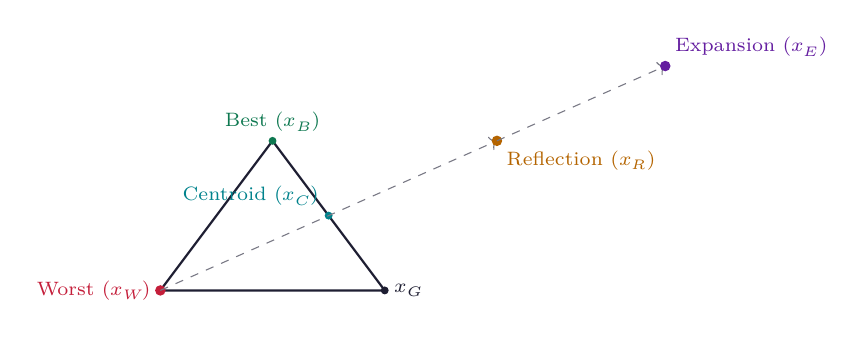
\begin{tikzpicture}[scale=0.95]
  % Define Vertices
  \coordinate (W) at (0,0); % Worst
  \coordinate (G) at (3,0); % Good
  \coordinate (B) at (1.5,2); % Best
  
  % Centroid of G and B
  \coordinate (C) at (2.25,1);
  
  % Simplex triangle
  \draw[thick, color=mydark] (W) -- (G) -- (B) -- cycle;
  \fill[myred] (W) circle (2pt) node[left, font=\scriptsize] {Worst ($x_W$)};
  \fill[mydark] (G) circle (1.5pt) node[right, font=\scriptsize] {$x_G$};
  \fill[mygreen] (B) circle (1.5pt) node[above, font=\scriptsize] {Best ($x_B$)};
  \fill[myteal] (C) circle (1.5pt) node[above left, font=\scriptsize] {Centroid ($x_C$)};
  
  % Operations
  % Reflection: x_R = x_C + (x_C - x_W)
  \coordinate (R) at (4.5,2);
  \draw[dashed, ->, color=mydark!60] (W) -- (R);
  \fill[myamber] (R) circle (2pt) node[below right, font=\scriptsize] {Reflection ($x_R$)};
  
  % Expansion: x_E = x_C + 2(x_C - x_W)
  \coordinate (E) at (6.75,3);
  \draw[dashed, ->, color=mydark!60] (R) -- (E);
  \fill[mypurple] (E) circle (2pt) node[above right, font=\scriptsize] {Expansion ($x_E$)};
\end{tikzpicture}
\end{tcolorbox}

\subsection{Hooke-Jeeves Pattern Search Method}
Hooke-Jeeves is a conceptual search method consisting of two primary components:
\begin{enumerate}[label=\textbf{\arabic*.}, leftmargin=*, itemsep=2.5pt]
  \item \textbf{Exploratory Move:} Performs local searches along the coordinate axes to find a direction of descent.
  \item \textbf{Pattern Move:} Performs an accelerated step along the direction established by connecting successive base points, bypassing slow orthogonal paths.
\end{enumerate}

% ===============================================================================
\section{Gradient-Based Descent Methods}
% ===============================================================================

\subsection{Cauchy's (Steepest Descent) Method}
Steepest descent moves in the direction of the local negative gradient vector, which represents the direction of maximum rate of decrease of the function.

\begin{tcolorbox}[formulabox, title={Steepest Descent Formulation}]
The iterative update equation is:
\begin{equation}
  \mathbf{x}_{k+1} = \mathbf{x}_k - \alpha_k \nabla f(\mathbf{x}_k)
\end{equation}
Where:
\begin{itemize}[leftmargin=*, itemsep=2pt, topsep=0pt]
  \item $\nabla f(\mathbf{x}_k)$ is the gradient vector at step $k$.
  \item $\alpha_k$ is the step length, determined by solving a unidirectional line search problem:
    \begin{equation}
      \text{Minimize } f(\mathbf{x}_k - \alpha \nabla f(\mathbf{x}_k)) \quad \text{w.r.t. } \alpha
    \end{equation}
\end{itemize}
*Characteristics:* Simple to implement but exhibits slow convergence near the optimum due to orthogonal zig-zagging trajectories.
\end{tcolorbox}

\subsection{Newton's Multivariable Method}
Newton's method uses a second-order quadratic approximation of the objective function.

\begin{tcolorbox}[formulabox, title={Newton's Multivariable Update}]
\begin{equation}
  \mathbf{x}_{k+1} = \mathbf{x}_k - [H(\mathbf{x}_k)]^{-1} \nabla f(\mathbf{x}_k)
\end{equation}
Where $[H(\mathbf{x}_k)]^{-1}$ is the inverse of the Hessian matrix.
\par\vspace{3pt}
*Characteristics:* Converges quadratically (extremely fast near the optimum) but requires calculating and inverting the Hessian matrix at every step, which is computationally expensive for large systems.
\end{tcolorbox}

% ===============================================================================
\section{Multi-Objective and Pareto Optimization}
% ===============================================================================

In real-world engineering, we often optimize multiple conflicting objectives simultaneously (e.g., minimizing cost while maximizing safety).

\subsection{Pareto Dominance \& Optimality}
Instead of a single optimum, multi-objective optimization yields a set of trade-off solutions.

\begin{tcolorbox}[defbox, title={Definition of Pareto Dominance}]
A decision vector $\mathbf{x}_1$ is said to \textbf{dominate} $\mathbf{x}_2$ if:
\begin{enumerate}[label=\textbf{\arabic*.}, leftmargin=*, itemsep=2pt, topsep=0pt]
  \item $\mathbf{x}_1$ is no worse than $\mathbf{x}_2$ in all objectives.
  \item $\mathbf{x}_1$ is strictly better than $\mathbf{x}_2$ in at least one objective.
\end{enumerate}
A solution is \textbf{Pareto Optimal} if it is not dominated by any other feasible solution. The set of all Pareto optimal solutions in the objective space forms the \textbf{Pareto Front}.
\end{tcolorbox}

\begin{tcolorbox}[tikzbox, title={Pareto Optimal Front (Conflicting Objectives)}]
\centering
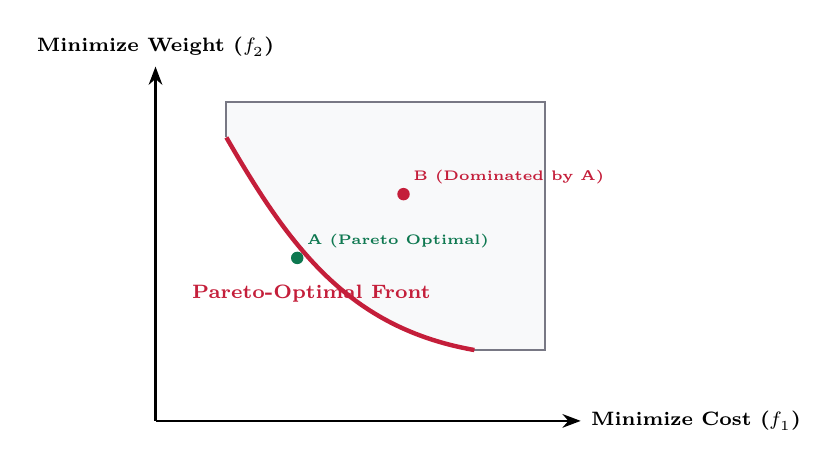
\begin{tikzpicture}[scale=0.9]
  \draw[-Stealth, thick] (0,0) -- (6,0) node[right, font=\scriptsize\bfseries] {Minimize Cost ($f_1$)};
  \draw[-Stealth, thick] (0,0) -- (0,5) node[above, font=\scriptsize\bfseries] {Minimize Weight ($f_2$)};
  
  % Feasible Region Shading
  \fill[mygray, opacity=0.8] (1,4) to[out=-60, in=170] (4.5,1) -- (5.5,1) -- (5.5,4.5) -- (1,4.5) -- cycle;
  \draw[thick, color=mydark!60] (1,4) -- (1,4.5) -- (5.5,4.5) -- (5.5,1) -- (4.5,1);
  
  % Pareto Curve
  \draw[ultra thick, color=myred] (1,4) to[out=-60, in=170] (4.5,1);
  \node[color=myred, font=\scriptsize\bfseries] at (2.2,1.8) {Pareto-Optimal Front};
  
  % Solution points
  \fill[mygreen] (2,2.3) circle (2.5pt) node[above right, font=\tiny\bfseries] {A (Pareto Optimal)};
  \fill[myred] (3.5,3.2) circle (2.5pt) node[above right, font=\tiny\bfseries] {B (Dominated by A)};
\end{tikzpicture}
\end{tcolorbox}

\newpage

% ===============================================================================
% MANDATORY QUICK REVISION PAGE
% ===============================================================================
\begin{center}
  {\large\bfseries\color{myred} Quick Revision --- Module 4}\\[3pt]
  {\small\color{mydark} Multivariable Optimization $|$ OE-EC704B}
\end{center}
\noindent{\color{myred}\rule{\linewidth}{1.2pt}}
\vspace{4pt}

\begin{tcolorbox}[formulabox, title={\textbf{Key Concepts \& Mathematical Rules}}]
\renewcommand{\arraystretch}{1.45}
\begin{tabularx}{\linewidth}{B{5.0cm} X}
Gradient Vector ($\nabla f$) & $\nabla f = \left[ \frac{\partial f}{\partial x_1}, \frac{\partial f}{\partial x_2}, \dots, \frac{\partial f}{\partial x_n} \right]^T = \mathbf{0}$. \\[4pt]
Hessian Matrix ($H$) & $H_{ij} = \frac{\partial^2 f}{\partial x_i \partial x_j}$ \quad (square symmetric matrix). \\[4pt]
Cauchy's Update & $\mathbf{x}_{k+1} = \mathbf{x}_k - \alpha_k \nabla f(\mathbf{x}_k)$ \quad (Steepest Descent). \\[4pt]
Newton's Update & $\mathbf{x}_{k+1} = \mathbf{x}_k - H^{-1} \nabla f(\mathbf{x}_k)$ \quad (Quadratic Convergence). \\[4pt]
Pareto Dominance Rule & $\mathbf{x}_1 \prec \mathbf{x}_2 \iff \forall i: f_i(\mathbf{x}_1) \le f_i(\mathbf{x}_2)$ and $\exists j: f_j(\mathbf{x}_1) < f_j(\mathbf{x}_2)$. \\
\end{tabularx}
\end{tcolorbox}

\begin{tcolorbox}[defbox, title={\textbf{One-Line Definitions}}]
\begin{itemize}[leftmargin=*, itemsep=2.5pt, topsep=0pt]
  \item \textbf{Positive Definite Matrix:} A matrix whose eigenvalues are all strictly positive (indicates local minimum structure).
  \item \textbf{Saddle Point:} A stationary point at which the Hessian matrix is indefinite (eigenvalues of mixed signs).
  \item \textbf{Nelder-Mead Simplex:} A derivative-free search method using vertices of a geometric figure to crawl toward the optimum.
  \item \textbf{Hooke-Jeeves Method:} A coordinate-based search method combining local exploratory moves and pattern acceleration.
  \item \textbf{Steepest Descent:} An iterative gradient method moving in the direction of the local negative gradient vector.
  \item \textbf{Pareto Front:} The set of all non-dominated solutions representing optimal trade-offs in multi-objective problems.
\end{itemize}
\end{tcolorbox}

\begin{tcolorbox}[exambox, title={\textbf{Frequently Asked / Viva Questions}}]
\begin{enumerate}[topsep=0pt, label=\textbf{Q\arabic*.}, itemsep=5pt]
  \item \Q{State the necessary and sufficient conditions for a local minimum of a multivariable function.}
    Necessary condition: The gradient vector must vanish, $\nabla f(\mathbf{x}^*) = \mathbf{0}$. Sufficient condition: The Hessian matrix $H(\mathbf{x}^*)$ must be positive definite.
  \item \Q{What is a Hessian matrix and what is its role in multivariable optimization?}
    The Hessian is a square symmetric matrix of second-order partial derivatives. Its role is to provide local curvature information to identify if a stationary point is a minimum, maximum, or saddle point.
  \item \Q{Explain why Cauchy's (Steepest Descent) method exhibits a zig-zag search trajectory.}
    Because successive search directions in Cauchy's method are mathematically orthogonal: $\mathbf{d}_k \cdot \mathbf{d}_{k-1} = 0$. This perpendicular stepping causes the algorithm to bounce back and forth in narrow valleys.
  \item \Q{What are the operations performed in the Nelder-Mead simplex search method?}
    The operations are Reflection, Expansion, Contraction (Outer and Inner), and Shrinkage.
  \item \Q{Differentiate between exploratory and pattern moves in the Hooke-Jeeves method.}
    An exploratory move searches along the coordinate axes to find a local descending direction. A pattern move accelerates the search by stepping along the vector connecting successive base points.
  \item \Q{Compare multivariable Newton's method with the Steepest Descent method.}
    Newton's method converges quadratically (very fast) but requires calculating and inverting the Hessian matrix. Steepest descent only requires the first-order gradient, making it computationally simpler per step but much slower to converge.
  \item \Q{What is Pareto optimality in multi-objective optimization?}
    A solution is Pareto optimal if no other solution exists that improves one objective without simultaneously degrading at least one other objective.
  \item \Q{Define the concept of a saddle point.}
    A saddle point is a stationary point where the gradient is zero, but the Hessian is indefinite, meaning the function increases in some directions and decreases in others.
  \item \Q{What is the purpose of a unidirectional line search in multivariable algorithms?}
    To find the optimal step length $\alpha_k$ that minimizes the function along the selected search direction $\mathbf{d}_k$: $\min_\alpha f(\mathbf{x}_k + \alpha \mathbf{d}_k)$.
  \item \Q{What makes a matrix positive definite using Sylvester's Criterion?}
    A symmetric matrix is positive definite if and only if all its leading principal minors (determinants of top-left submatrices) are strictly positive.
\end{enumerate}
\end{tcolorbox}

\end{document}
